
\shinyChapterQuote{If you do not want to use this thing,\newline comment out the contents of the command \newline \swCmd{\textbackslash shinyChapterQuote} in file \swCmd{styles/documentStyle.tex} to make empty output}
       {Florian Cordes}

\todo{adapt to your own thesis!}
This chapter provides a motivation for the thesis and defines the scope of the topics covered.
The contributions are outlined and the structure of the thesis with an overview of the chapters and related publications is presented in this chapter.
The chapter is closed with a content summary of the author's publications contributing to this thesis.


\section{Motivation and Scope}
\label{sec:Intoduction:Motivation}
\lipsum

\section{Thesis Contributions}
The main contribution of this thesis is 

\begin{figure}%[b]
%\vspace{-2ex}
  \centering
  \hypersetup{linkcolor=captionTextColor}
  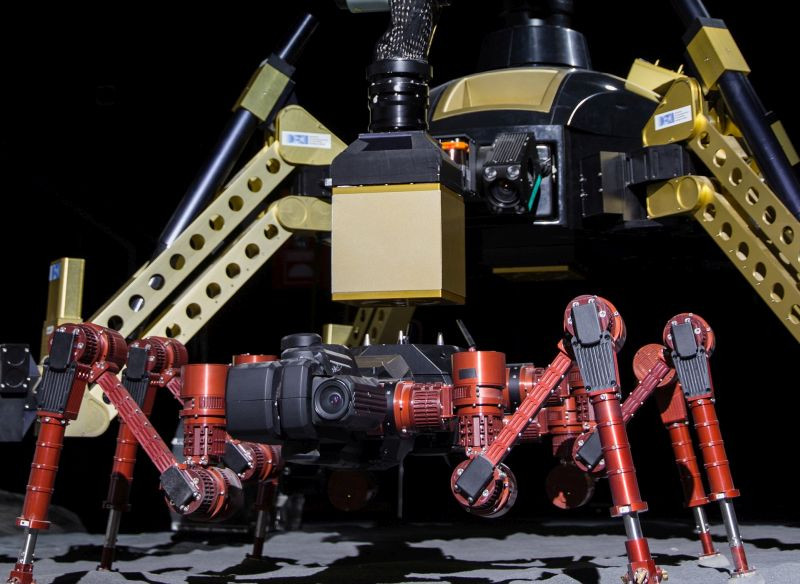
\includegraphics[width=0.8\linewidth]{pictures/RIMRES-final-14}\\
  %\vspace{-2ex}
  \caption[A sample image]
          {A sample image. This is a longer caption than that used for the index.}
  \label{fig:RIMRES-final-14}
  %\vspace{-3ex}
\end{figure}

\begin{figure}%[b]
\vspace{-2ex}
	\centering
    %% setup sizes
    \setlength{\subfigureWidth}{0.32\textwidth}
    \setlength{\graphicsHeight}{33mm}
    %% kill hyper-link highlighting
    \hypersetup{hidelinks=true}%
    %% the figures
	\begin{subfigure}[t]{\subfigureWidth}
        \centering
		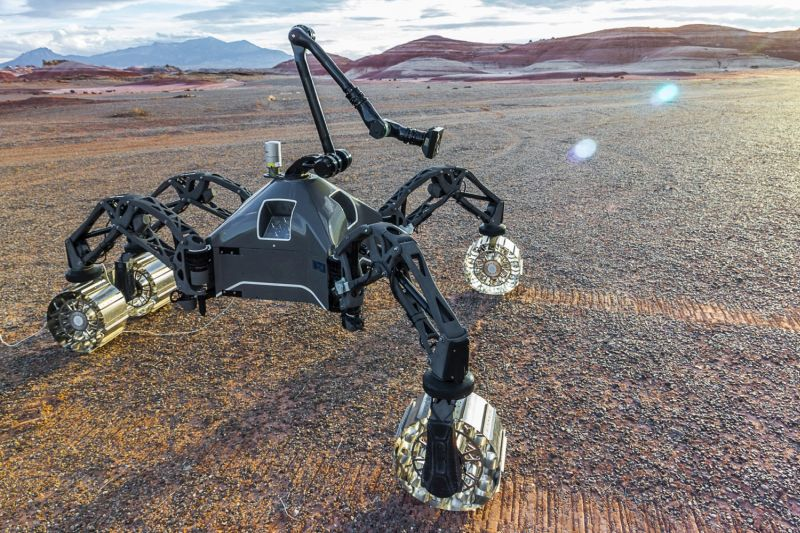
\includegraphics[height=\graphicsHeight]{pictures/SherpaTT_QuasiTripod}
		\subcaption{Quasi tripod pose}
		\label{fig:SherpaTT_QuasiTripod}
	\end{subfigure}\hfill
	\begin{subfigure}[t]{\subfigureWidth}
        \centering
		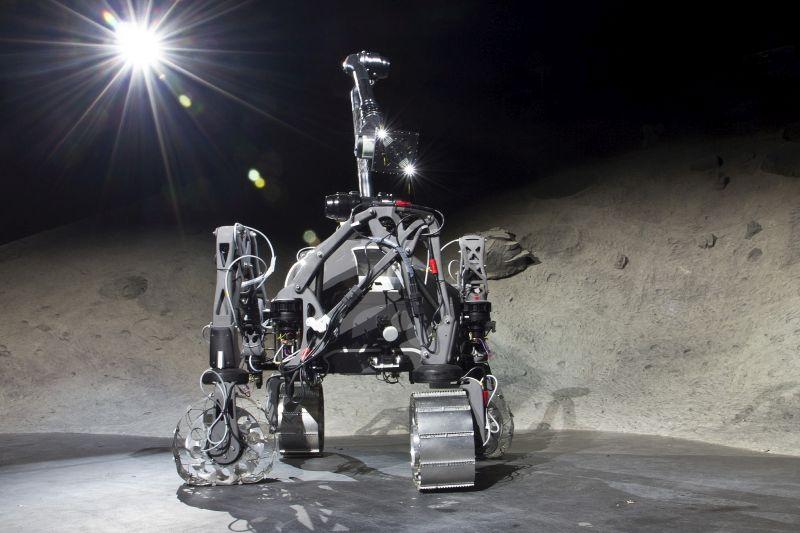
\includegraphics[height=\graphicsHeight]{pictures/SherpaTT_Stow}
		\subcaption{Compact stow pose of legs}
		\label{fig:SherpaTT_Stow}
	\end{subfigure}\hfill
    \begin{subfigure}[t]{\subfigureWidth}
        \centering
		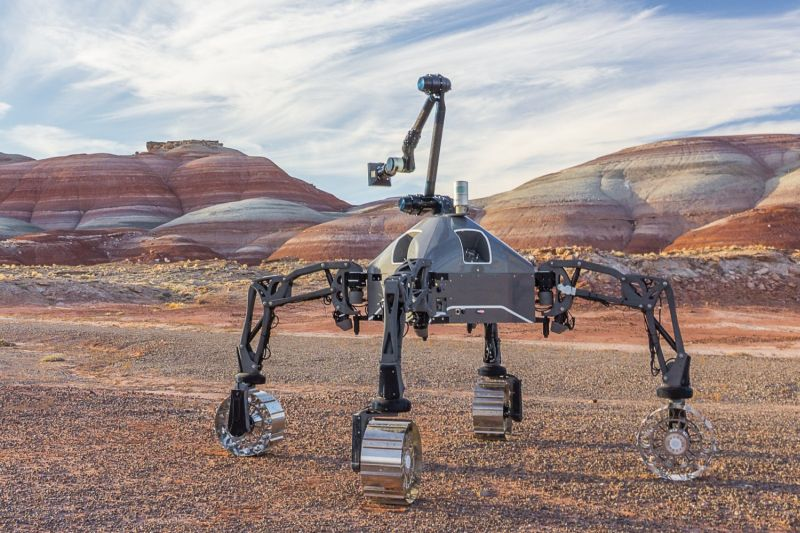
\includegraphics[height=\graphicsHeight]{pictures/SherpaTT_HighPose}
		\subcaption{High body pose in CrossStance}
		\label{fig:SherpaTT_HighPose}
	\end{subfigure}\\[0.8ex]
%% 2nd row
    \begin{subfigure}[t]{\subfigureWidth}
        \centering
		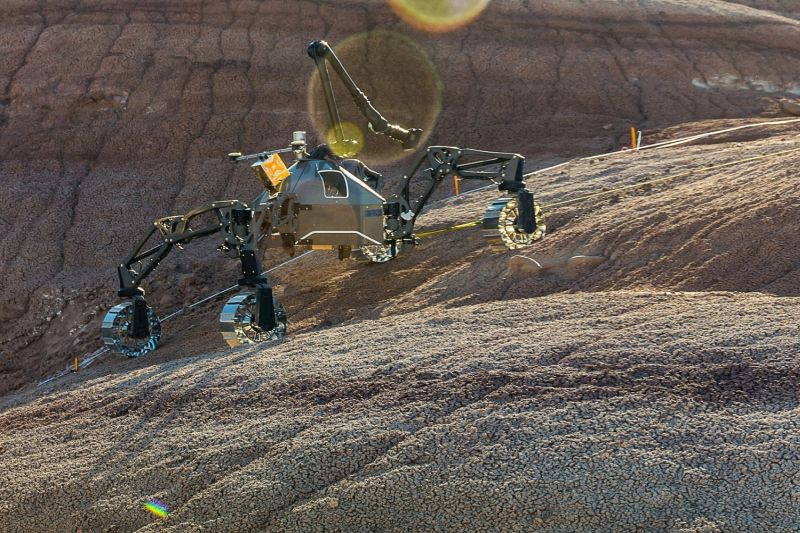
\includegraphics[height=\graphicsHeight]{pictures/SherpaTT_RPA_Utah}
		\subcaption{Body roll-pitch control in sloping natural terrain}
		\label{fig:SherpaTT_RPA_Utah}
	\end{subfigure}\hfill
	\begin{subfigure}[t]{\subfigureWidth}
        \centering
		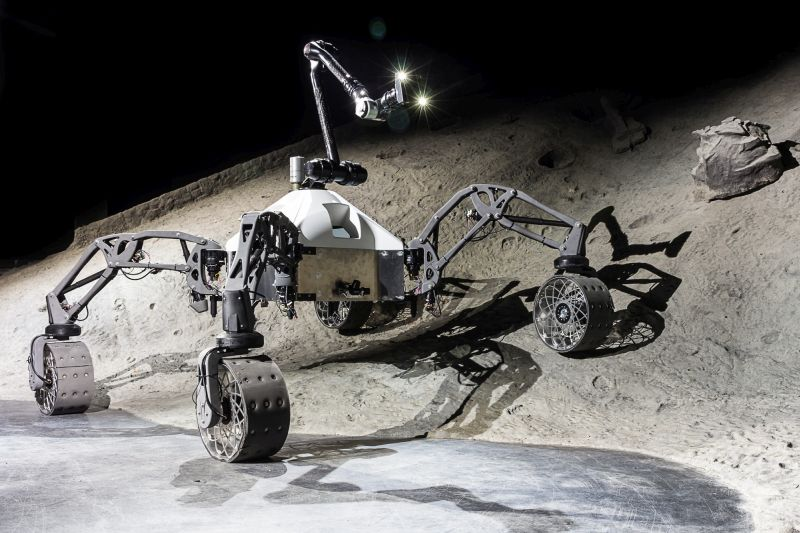
\includegraphics[height=\graphicsHeight]{pictures/SherpaTT_RPA_Crater}
		\subcaption{Body roll-pitch control in artificial crater}
		\label{fig:SherpaTT_RPA_Crater}
	\end{subfigure}\hfill
    \begin{subfigure}[t]{\subfigureWidth}
        \centering
		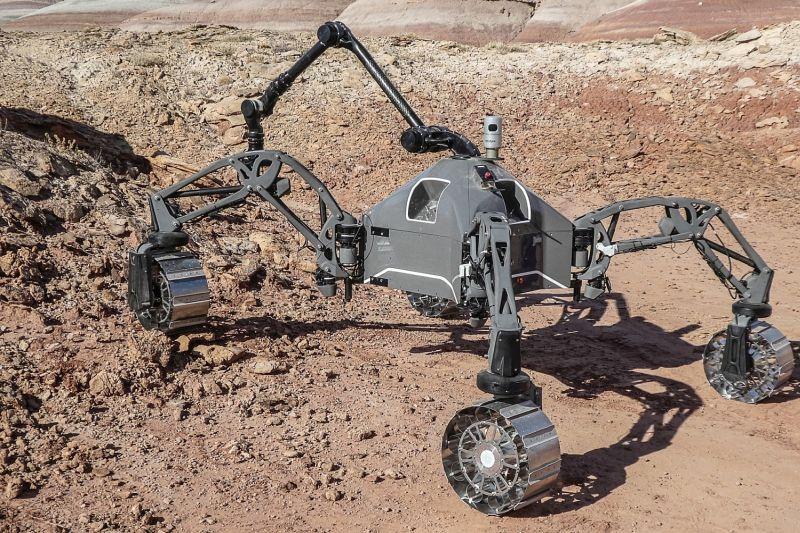
\includegraphics[height=\graphicsHeight]{pictures/SherpaTT_SamplingUtah}
		\subcaption{Approaching a sampling spot in natural terrain}
		\label{fig:SherpaTT_SamplingUtah}
	\end{subfigure}
	\caption{Example of a figure with subfigures}
	\label{fig:SherpaTT}
\vspace{-2ex}
\end{figure}


\begin{table}%[h]
%\vspace{-2ex}
  %\centering
  \hypersetup{hidelinks=true}
  %
  \caption[Exemplary table]{Exemplary table.
  \dissExtraCaption{With an example of an extra caption. Should be used with optional caption.}
  }
  \label{tab:Design:ComparisonSherpaSherpaTT}
  \begin{footnotesize}
      \begin{tabular}{l| rrr r ll r rr}
        \toprule
         \rowcolor{tableheadingcolor}
        System  & Leg length & Mass    & Mass & \ac{DoF}         & vert. & horz. & min stow  & \multicolumn{2}{c}{compactness}\\
        \rowcolor{tableheadingcolor}
                & zero pose &  (leg)  & total  & (leg)   & stroke &  stroke &volume    & footprint & volume \\
        \midrule
        \cellcolor{tablesubheadingcolor}Sherpa      & 976\unitmm & 25\unitkg & 160\unitkg &6          & 900\unitmm
%        \color{captionTextColor}{$^{\ast}$}
        & 260\unitmm
%        \color{captionTextColor}{$^{\ast\ast}$}
        &  2.24\unitcubmeter & 0.40 & 0.64\\
        \cellcolor{tablesubheadingcolor}SherpaTT\hspace{-1mm}    & 977\unitmm & 26\unitkg & \massSherpaTT &5          & 775\unitmm & 485\unitmm & 1.67\unitcubmeter & 0.79 & 0.72\\
        \bottomrule
      \end{tabular}
  \end{footnotesize}
\end{table}





\section{Structure of Thesis}
The structure of this thesis is illustrated in \refFig{fig:structure_diagram}. \todo{if you do not want to use citations, check \swCmd{styles/structureGraphFunctions.tex} with the example of an alternative \swCmd{\textbackslash drawChapterBox} command}
From the publications forming this cumulative thesis, those related to each chapter are provided in the respective box.
Further publications of the author are cited at the appropriate places in each paragraph.



\begin{figure}%[htb]
    \begin{center}
        %%%%%%%%%%%%%%%%%%%%%%%%%%%%%%%%%%%%%%%%
%%% structural graph of thesis document
%%%%%%%%%%%%%%%%%%%%%%%%%%%%%%%%%%%%%%%%


%% helper for minipages
%%  \begin{minipage}[outerPos][height][innerPos]{width}
%%	     Beispieltext
%%  \end{minipage}
%% outerPos (optional; c,t,b): where the minipage is on the page (center, top, bottom)
%% height (optional): height o minipage, regardless of contents
%% innerPos (optional; c,t,b): where the content is (center, top, bottom)

% set some dimension variables for minipages
\newlength{\structureGraphHeight}
\setlength{\structureGraphHeight}{100mm}

\newlength{\chapterboxWith}
\setlength{\chapterboxWith}{0.45\linewidth}

\newlength{\chapterboxHeight}
\setlength{\chapterboxHeight}{21mm}





%%% the actual graph







%%%%%%%%%%%%%%%%%%%%%%%%%%%%%%%%%%%%%%%%%%%%%%%%%%%%%%%%%%%%%%%%%%%%%%%%%%%%%%%%%%%%%%%%%%%%%%%%%%%%%%%%%%%%%
%% this is the actual structure plot
%% settings are in   thesis_colors.sty   and   styles/structrueGraphFunctions.tex
%%



%\begin{tcolorbox}[code={\pgfkeysalsofrom{\outerboxoptions}},
%                  title=Thesis: \newline\qq{\myWorkingTitle}]
    %external raster
    \begin{tcbraster}[ code={\pgfkeysalsofrom{\outerrasteroptions}} ]
            %ROW 1                                                        % |-- SINGLE-box-Options
            \partbox{Intro}{}{                                            % v
                \begin{tcboxedraster}[ code={\pgfkeysalsofrom{\innerrastersinglecoloptions}} ]{blankest}
                        \rule{0.25\linewidth}{0pt}% remove for dual
                        \drawChapterbox{sec:introduction}{\introCites}%
                        %\rule{0.2\linewidth}{0pt}%
                \end{tcboxedraster}
            }
            % ROW2
            \partbox{Foundations}{}{
                \begin{tcboxedraster}[ code={\pgfkeysalsofrom{\innerrasterdualcoloptions}} ]{blankest} 
                        \drawChapterboxSota{sec:sota}{ \sotaCites }%
                        \drawChapterbox{sec:ReqirementsConditions}{ ~ }%
                \end{tcboxedraster}
            }
            % ROW3                                                       % |-- DUAL-box-Options
            \partbox{Design}{}{                                          % v
                \begin{tcboxedraster}[ code={\pgfkeysalsofrom{\innerrasterdualcoloptions}} ]{blankest} %<- no drawn box or white space around inner boxes
                        \drawChapterbox{sec:RobotDesign}{ \designCites }%
                        \drawChapterbox{sec:control}{ \controlCites }%
                \end{tcboxedraster}
            }
            %ROW 4
            \partbox{~~Experi-}{mentation}{
                \begin{tcboxedraster}[ code={\pgfkeysalsofrom{\innerrastersinglecoloptions}} ]{blankest}
                        \rule{0.25\linewidth}{0pt}%
                        \drawChapterbox{sec:Experiments}{ \expCites }%
                        %\rule{0.2\linewidth}{0pt}%
                \end{tcboxedraster}
            }
            %ROW 5
            \partbox{Conclusion}{}{
                \begin{tcboxedraster}[ code={\pgfkeysalsofrom{\innerrastersinglecoloptions}} ]{blankest}
                        \rule{0.25\linewidth}{0pt}%
                        \drawChapterbox{sec:ConclusionOutlook}{ \conclusionCites }%
                        %\rule{0.2\linewidth}{0pt}%
                \end{tcboxedraster}
           }
            %ROW 6
            \partbox{Appendix}{}{
                \begin{tcboxedraster}[ code={\pgfkeysalsofrom{\innerrastertriplecoloptions}} ]{blankest}
                        %\rule{0.25\linewidth}{0pt}%
                        \drawAppendixbox{sec:Appendix:AdditionalMaterial}{ ~ }%
                        \drawAppendixbox{sec:Appendix:MoreStuff}{ ~ }%
                        \drawAppendixbox{sec:Appendix:Enough}{ ~ }%
                        %\rule{0.2\linewidth}{0pt}%
                \end{tcboxedraster}
            }
    \end{tcbraster}
%\end{tcolorbox}	














    \end{center}
    \vspace{-1ex}
    \caption{Structure of this thesis and related publications per chapter.}
    \label{fig:structure_diagram}
    %\vspace{-1.8ex}
\end{figure}


\section{Bibliography Remarks}
\label{sec:intro:BibRemarks}
\todo{run the \swCmd{make\_bib.bat} file or the command lines within to generate the bibliography}
To better distinguish between the author's own publications and citations from literature, different citation marks are applied:
\begin{compactitem}
  \item Citations from the author's own publications are plain numbered, \eg~\citeown{myPubA}, \citeown{myPubB}. 
  \item Citations from literature are using the author-year format, \eg~\citesota{Wilcox2012}.
\end{compactitem}



